\documentclass[11pt,a4paper]{article}
\usepackage{times}
\usepackage{latexsym}
\usepackage{graphicx}
\usepackage{natbib}
\usepackage{amsmath}
\usepackage{amsfonts}
\usepackage{bm}
\usepackage{multirow}
\usepackage[linesnumbered, boxed, ruled]{algorithm2e}
\newcommand{\KZ}[1]{\textcolor{blue}{Kenny: #1}}
\renewcommand\arraystretch{1.2}
\setlength\parskip{0.1\baselineskip}
\setlength{\textfloatsep}{0.5cm}
% This is not strictly necessary, and may be commented out,
% but it will improve the layout of the manuscript,
% and will typically save some space.
\usepackage{microtype}
\newcommand{\secref}[1]{Section \ref{#1}}
\newcommand{\figref}[1]{Figure \ref{#1}}
\newcommand{\eqnref}[1]{Eq. (\ref{#1})}
\newcommand{\tabref}[1]{Table \ref{#1}}
\newcommand{\exref}[1]{Example \ref{#1}}
\newcommand{\cut}[1]{}

\usepackage{tikz}
\usepackage{geometry}
\usetikzlibrary{automata,positioning}
\geometry{left=2.0cm, right=2.0cm, top=2.5cm, bottom=2.5cm}


\title{xxxx}

\date{}


\begin{document}

\appendix
\section{Base Models}
\label{ap:datastats}
\subsection{CrossAlign}
The \emph{CrossAlign} model architecture proposed by \citet{shen2017style} is shown in \figref{fig:crossalign}. Let $X$ and $Y$ be two corpus with styles $s_x$ and $s_y$, respectively. $E$ is the encoder that takes source sentence $x$/$y$ and style label $s_x$/$s_y$ as input. The encoded entangled embedding $z_x$/$z_y$ is then combined with its source style label $s_x$/$s_y$ as input to the decoder $D$ to reconstruct the input sentence. Two adversarial discriminators $D_1$ and $D_2$ are introduced to distinguish the hidden state sequence of $D(z_x, s_x)$/$D(z_y, s_y)$ between the hidden state sequence of $D(z_y, s_x)$/$D(z_x, s_y)$, respectively.

\begin{figure}[htbp]
	\centering
	\scalebox{1.2}{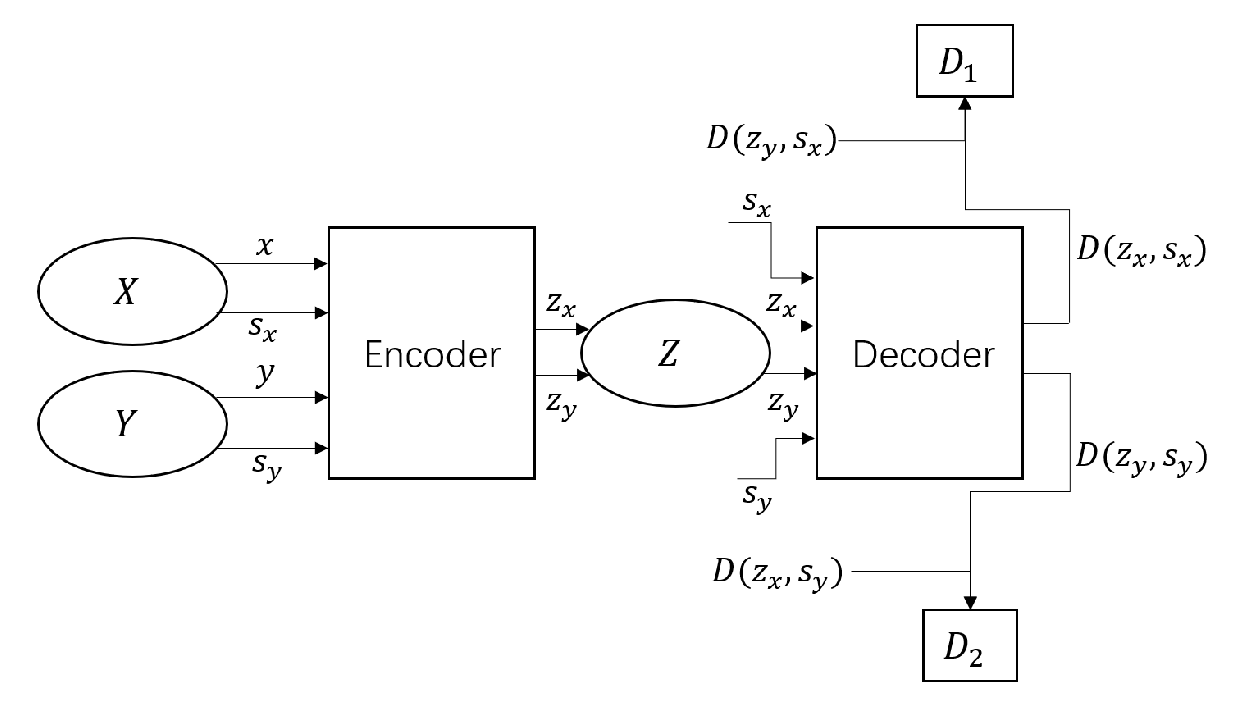
\includegraphics[width=7cm]{./images/cross_align_new_new.eps}}
	\caption{CrossAlign architecture}
	\label{fig:crossalign}
\end{figure}

In training phase, the discriminators and the encoder-decoder model are optimized in an alternate fasion. The objective is to find
\begin{align*}
\theta^* = \underset{\theta}{\arg\min\ } \mathcal{L}_{\mathrm{rec}} (\theta_E, \theta_D) &- \mathcal{L} _{\mathrm{adv}}(\theta_E, \theta_{D},\theta_{D_1}) \\
&- \mathcal{L}_{\mathrm{adv}}(\theta_E, \theta_D,\theta_{D_2}),
\end{align*}
where
\begin{align*}
\mathcal{L}_{\mathrm{adv}}(\theta_E, \theta_D,\theta_{D_1}) & = \mathbb{E}_{x\sim X}[-\log D_1(D(E(x, s_x),s_x))] & \\
+ &\mathbb{E}_{y\sim Y}[-\log (1 - D_1(D(E(y, s_y), s_x)))],\\
\mathcal{L}_{\mathrm{adv}}(\theta_E, \theta_D,\theta_{D_2}) & = \mathbb{E}_{y\sim Y}[-\log D_2(D(E(y, s_y),s_y))] & \\
+ &\mathbb{E}_{x\sim X}[-\log (1 - D_2(D(E(x, s_x), s_y)))]
\end{align*}
The discriminators $D_1$ and $D_2$ are both implemented as CNN classifiers~\citep{kim2014convolutional}.

\subsection{VAE for Style Transfer}
In order to disentangle style and content in the latent space, \citet{john2018disentangled} used variational autoencoder (VAE) and their specially designed style-oriented and content-oriented losses to guide the updates of the latent space distributions for the two components~\citep{kingma2013auto}. 

The architecture of this model is shown in \figref{fig:vae}. Given a corpus $X$ with unknown latent style space and content space, 
an RNN encoder maps a sequence $x$ into the latent space, 
which defines a distribution of style and content~\citep{cho2014learning}. 
Then style embedding and content embedding are sampled from 
their corresponding latent distributions and are concatenated 
as the training sentence embedding. 

The two embeddings are used to calculate multi-task 
loss $J_{\mathrm{mul}}$ and adversarial loss $J_{\mathrm{adv}}$ 
for content and style to separate their information. 
Then this concatenated latent vector is used as a generative 
latent vector, and is concatenated to every step of the input sequence
and fed into decoder $D$, which reconstructs the sentence $x'$. 
The final loss is the sum of these multi-task losses and the usual VAE reconstruction $J_{\mathrm{rec}}$ with 
KL divergence regularization for both style embedding and content 
embedding~\citep{kingma2013auto}.

\begin{figure}[htbp]
	\centering
	\includegraphics[width=7cm]{./images/vae.pdf}
	\caption{VAE architecture}
	\label{fig:vae}
\end{figure}

In the training phase, the adversarial discriminators are trained 
together with other parts of the model, and the final loss of 
the autoencoder is given by the weighted sum of the loss from traditional VAE, 
the multitask losses for style and content, 
and the adversarial losses given by the style and content discriminators. 
In the inference phase, the style embedding is extracted from the 
latent space of a target domain and then combined with the original content embedding as input to the decoder.
%Table \ref{tb:datastats} shows the vocabulary size, average sentence length, number of adjectives and Flesch readability of our two datasets. For each dataset, we only selected a specific pair of styles, which are Michael R. Katz/Richard Pevear for LT, and simple/standard Wikipedia for GSD. (Flesch readability ranges from 0 to 100, with higher meaning easier to read.)
%
%\begin{table*}[th]\footnotesize
%	\centering
%	\begin{tabular}{c|cccc}
%		& Vocab Size & Avg. Length & \#. of Adj. & Flesch \\
%		\hline
%		LT & 12589 / 13643 & 19.8 / 21.3 & 15338 / 13623 & 65.1 / 66.2 \\
%		GSD & 18124 / 20112 & 11.1 / 11.8 & 10692 / 12070 & 58.5 / 52.3
%	\end{tabular}
%	\caption{Dataset characteristics.}\label{tb:datastats}
%\end{table*}

%\section{More Generated Samples}
%
%Table \ref{tb:qualmore} lists some more samples that are randomly selected from the generated sentences of all models.
%
%\begin{table*}[th]\footnotesize
%	\centering
%	\begin{tabular}{c|c}
%		\hline
%		\textbf{Original Sentence} (Yelp positive) & \emph{the staff is welcoming and professional .} \\
%		\hline
%		Template & \emph{the staff is welcoming and professional .} \\
%		CrossAlign & \emph{glad glad glad} \\
%		CrossAlign (pretrained) & \emph{the staff is welcoming and professional .} \\
%		DeleteRetrieve & \emph{the staff is a time .} \\
%		DualRL & \emph{less expensive have working .} \\
%		VAE & \emph{the staff is rude and rude} \\
%		VAE (pretrained) & \emph{the staff is extremely welcoming and professional .} \\
%		\hline
%		ST$^2$-CrossAlign (ours) & \emph{the staff is friendly and unprofessional} \\
%		ST$^2$-VAE (ours) & \emph{the staff are rude and unprofessional .} \\
%		\hline
%		\hline
%		\textbf{Original Sentence} (Yelp negative) & \emph{these people do not care about patients at all !} \\
%		\hline
%		Template & \emph{these people wonderful about patients at all !} \\
%		CrossAlign & \emph{glad glad glad} \\
%		CrossAlign (pretrained) & \emph{these people do not care about patients at all !} \\
%		DeleteRetrieve & \emph{i was n't be a a appointment and i have .} \\
%		DualRL & \emph{and just like that it was over and i was .} \\
%		VAE & \emph{these people do not care about patients or doctors} \\
%		VAE (pretrained) & \emph{these guys do n't care about the patients at time} \\
%		\hline
%		ST$^2$-CrossAlign (ours) & \emph{these people do not satisfied at all !} \\
%		ST$^2$-VAE (ours) & \emph{i was so happy and i did n't consent} \\
%		\hline
%	\end{tabular}
%	\caption{Randomly selected sample outputs for the Yelp positive/negative review dataset.}\label{tb:qualmore}
%\end{table*}
\subsection{CP-VAE}
\citet{Xu2019} found that traditional squence VAEs trained on text often fail to decode the inferred latent codes because the manipulated latent codes tend to land in hole or vacant regions in latent space being modeled. To mitigate the problem, they proposed to constrain the latent space within a learned probability simplex by projecting the encoded original Gaussian mean to a probability distribution over a set of basis vectors, which are also learned during training.
The core difference between CP-VAE and conventional VAEs is the following constraint of posterior mean:
\begin{equation}
	 \bm{u}= \pi(\bm{h}) = \bm{E} \cdot softmax(\bm{Wh}+\bm{b})
\end{equation}
Where $\bm{E}$ is the learned basis vectors $\bm{e}_i$, $i=1,...,K$~($K\ll N$), $N$ is the dimensionality of latent space. To encourage orthogonality in the basis vectors, a regularization term is added to the training objective:
\begin{equation}
	\mathcal{L}_{REG}=\|\bm{E}^T\bm{E}-\alpha \bm{I}\|
\end{equation}
To decide which basis vector corresponds to which style, a set of samples from validation set is extracted and used to compute the probability $\bm{p}=\bm{E}\cdot softmax(\bm{Wh}+\bm{h})$ over basis vectors. The basis vector with highest probability is then fixed as the latent code and passed to decoder to generate the target sentence.
\bibliography{style}
\bibliographystyle{aaai21}
\end{document}
